\documentclass[8pt]{beamer}
\usepackage{amsmath}
\usepackage{amssymb}
\usepackage{graphicx}
\usepackage{hyperref}
\usepackage{color}
\usepackage{float}
\usepackage{subfig}

\title{Peak detection using positive False Discovery Rate\\
Applications in chromosome capture data}
\author{Ofir Shukron}
\usetheme{Madrid}
\usecolortheme{dolphin}
\begin{document}

\begin{frame}
\titlepage
\end{frame}

\begin{frame}{Motivation}
\begin{enumerate}
\item Multiple hypotheses are being tested on large amount of experimental data. 
\item Many time it is required to find outlying observations (peaks). 
\item When finding many peaks, a criteria to control the error rate is needed.
\item One would like to reduce type I errors. 
\item Restrictive traditional methods controlled the probability of at least one type I error.
\item New method of controlling the error called positive False Discovery Rate (pFDR) was developed\footnote{Storey JD. A direct approach to false discovery rates. J. R. Statist. Soc. B (2002)64, Part 3, pp. 479–498}. 
\item We want to apply this method to find frequent specific looping events in the chromosomes using chromosome capture (CC) data.
\item Under the assumption of a polymer model, the peaks will be treated individually in the reconstruction of polymer structure from encounter data.
\end{enumerate}
\end{frame}

\begin{frame}{A simple model}

 Assuming $n$ realizations of a process $R(d)\in \mathcal{C}^0,\quad d\in\mathbb{R}$ with noise term $F(d)=\{f_1(d),f_2(d),...,f_n(d)\}, \quad f_i\sim \mathcal{N}(0,1)\quad \forall i$, such that 
 \begin{equation*}
 s_i(d) = R(d)+\sigma f_i(d),\qquad i=1..n
 \end{equation*}
 
 Assume $\Lambda=\{\lambda_1,\lambda_2,...,\lambda_n\}$ are $n$ realizations of a random pulse process, e.g characterized by $\lambda_i(d)\sim Bin(1,p\ll1)$ such that, 
 \begin{equation*}
 s_i(d)=R(d)+\sigma f_i(d)(1+c\lambda_i(d))
 \end{equation*}
  with $c=const$
\begin{figure}[H]
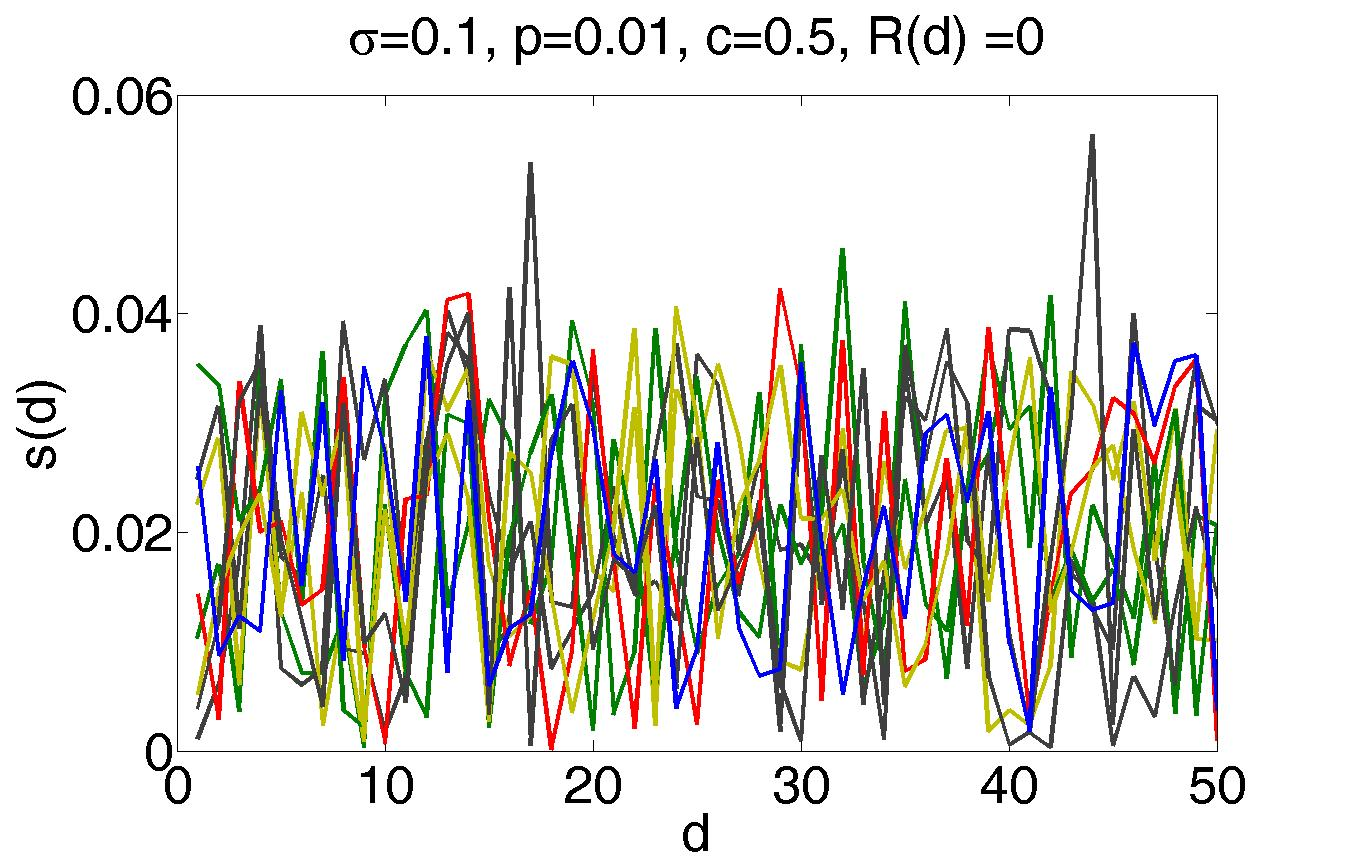
\includegraphics[scale=0.08]{randSignalSample}
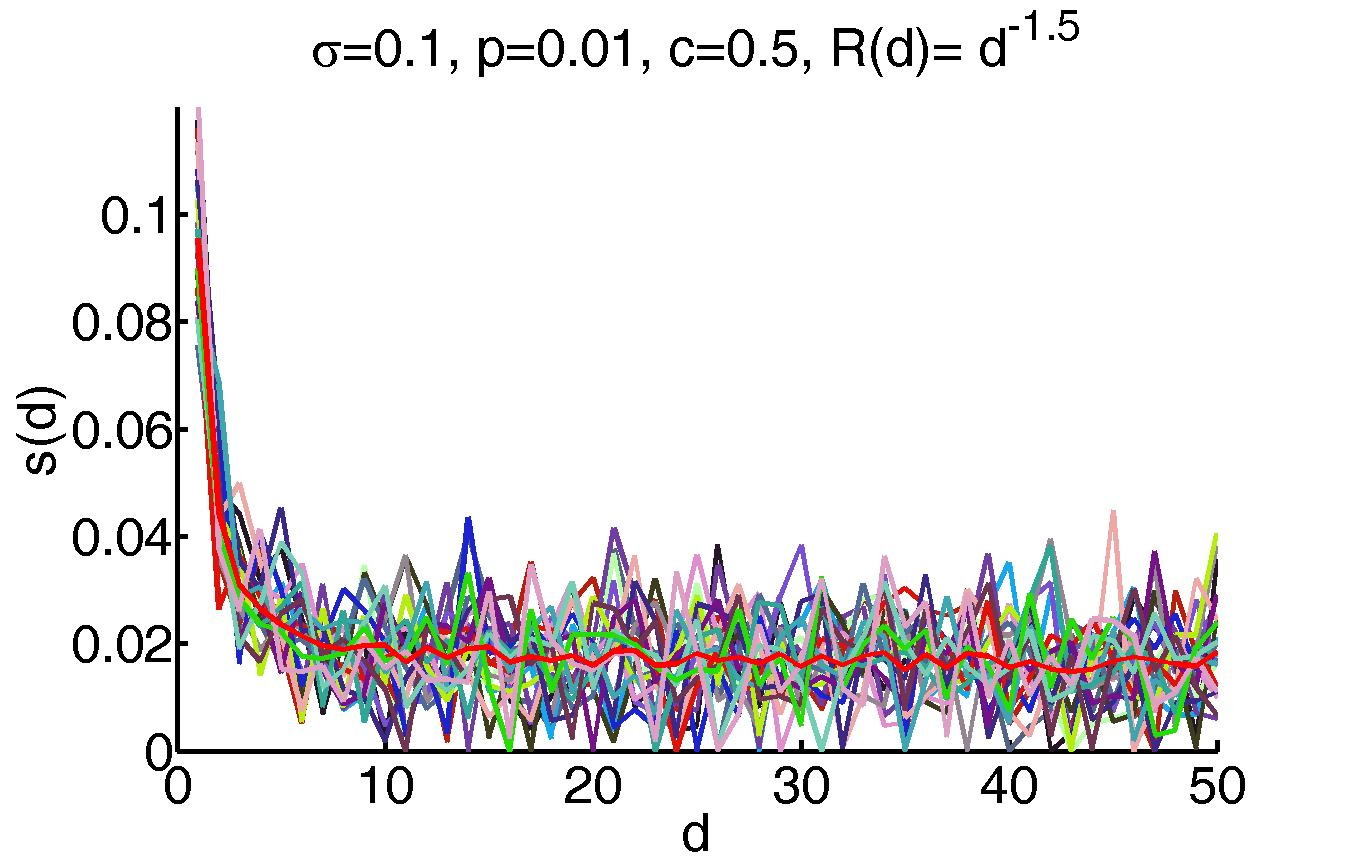
\includegraphics[scale=0.08]{gaussianChainSignalSample}
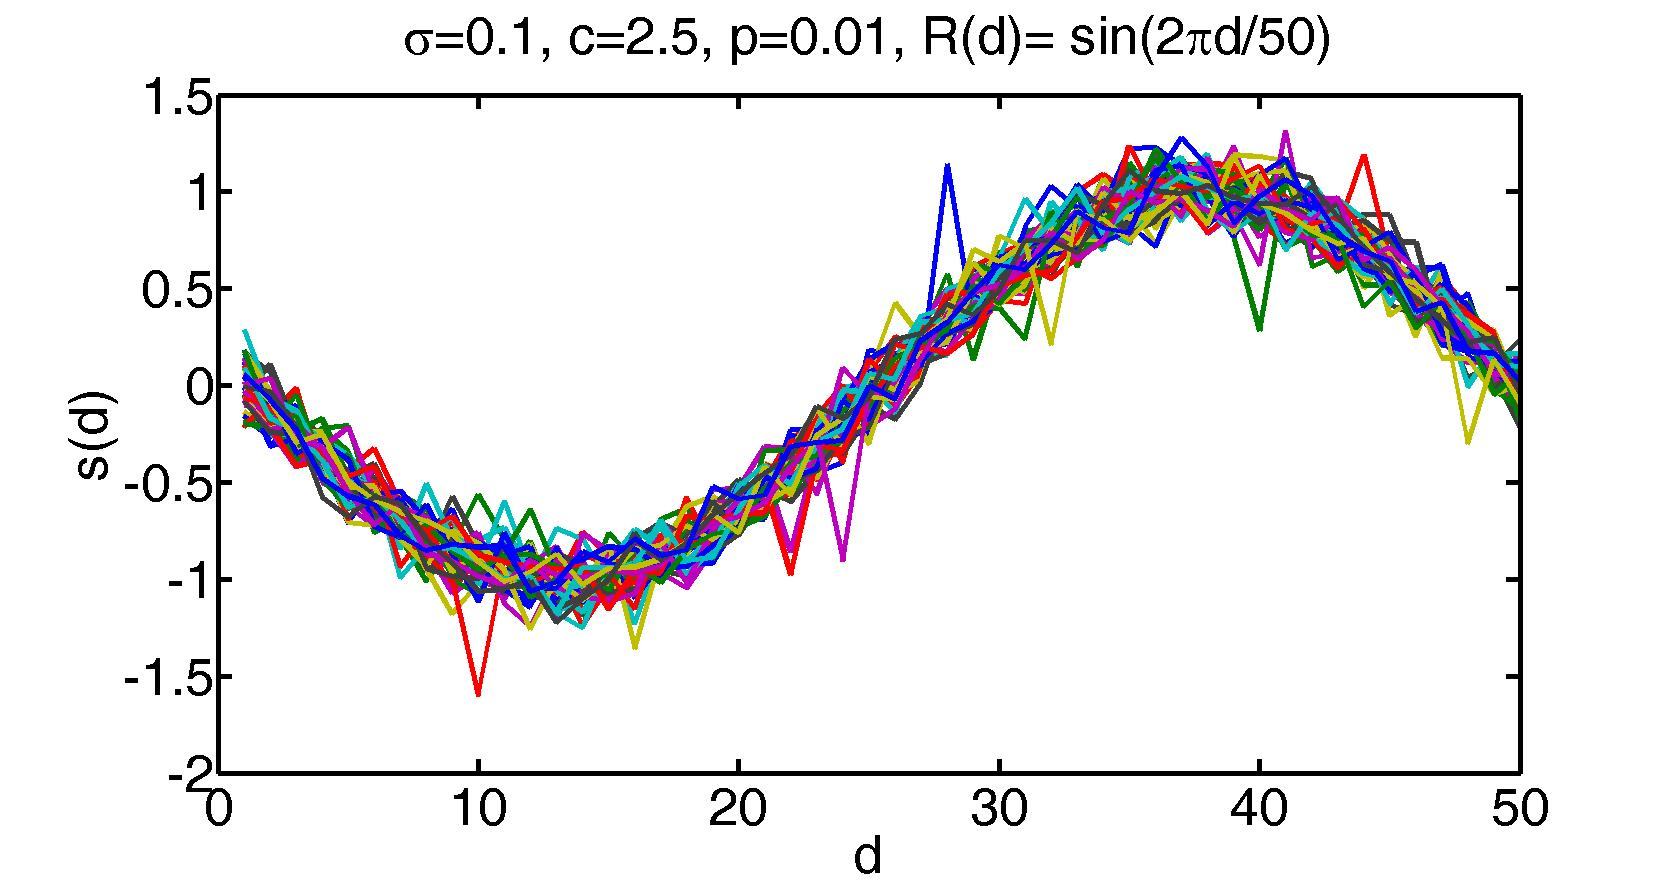
\includegraphics[scale=0.08]{sinSignalSample}
\end{figure}

\end{frame}

\begin{frame}{Approach}
\begin{enumerate}
\item Estimate the expected signal and signal density (parametric or empirical) and set rejection region (value) $\Gamma$.
\item Calculate signals' densities for each $d$ and p-values according to the rejection region.
\item Reminder: $p-value(t) = \min_{\{\Gamma;t\in\Gamma\}}\{Pr(T\in\Gamma |H=0)\}$
\item Shrink the rejection region to reduce type I errors/balance Type II errors.
\end{enumerate}

\begin{figure}[H]
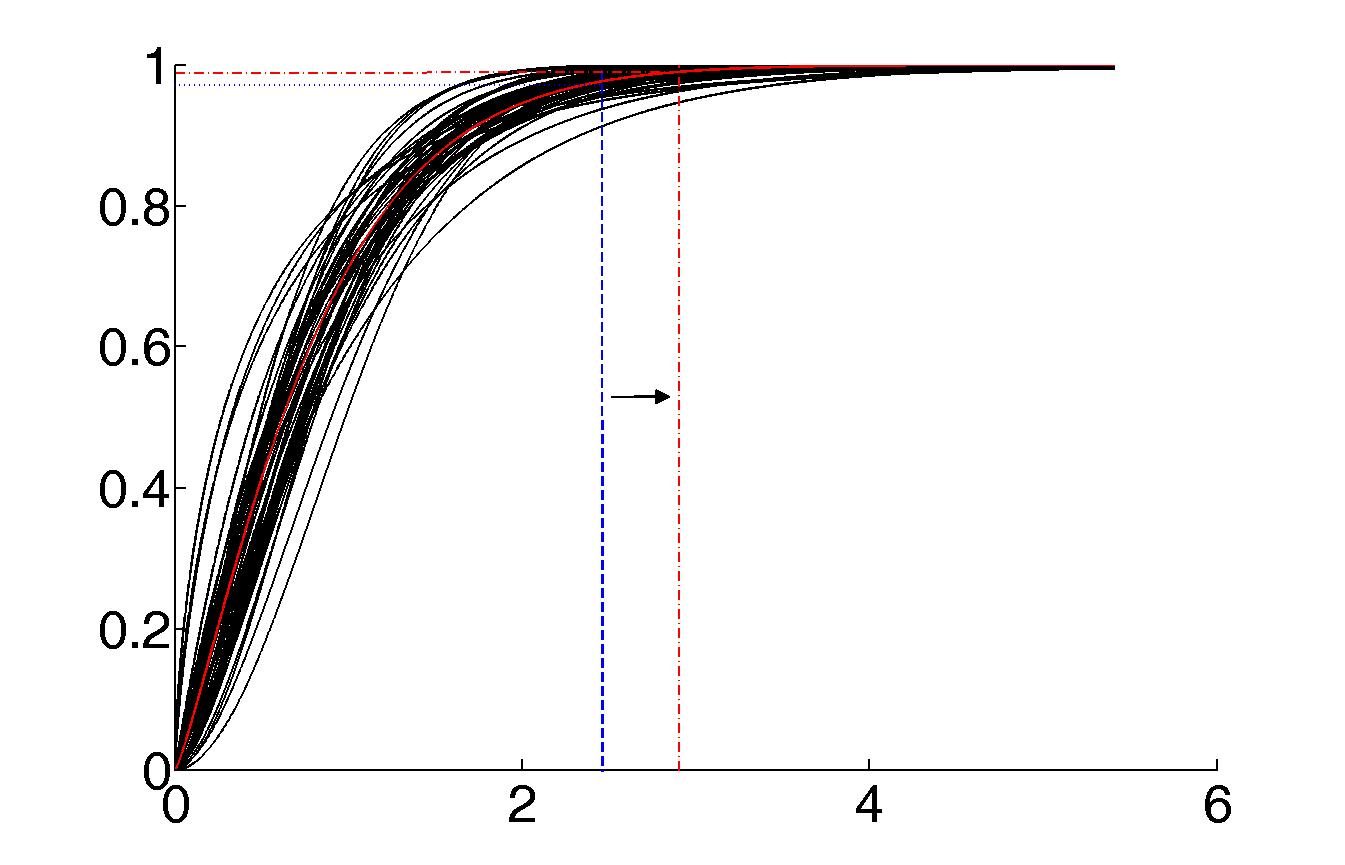
\includegraphics[scale=0.15]{rejectionValueAdjastmentScheme}
\end{figure}
\end{frame}

\begin{frame}{Mathematical derivation}
Conducting $m$ hypothesis tests, using p-values, $P$, as our test statistics.\\
We fix a rejection region $\gamma=[0, \gamma]$, and we reject the null hypothesis $H$ is $P\leq\gamma$. $(\gamma>0)$\\
Let $V$ be the number of type I errors and $R$ the total number of rejections.\\
The pFDR is defined as: 
\begin{equation*}
pFDR=E\left(\frac{V}{R}| R>0 \right)
\end{equation*}

We assume that the null hypothesis $H$ is true ($H=0$) with an a priori probability $\pi_0$ and false ($H=1$) with probability $\pi_1$. We write (Storey 2001, Theorem 1)\\
\begin{equation*}
pFDR=\frac{\pi_0 Pr(P\leq\gamma|H=0)}{Pr(P\leq\gamma)}
\end{equation*}
By the Bayes rule 
\begin{equation*}
pFDR = Pr(H=0|P\leq\gamma)
\end{equation*}

Under the null hypothesis, the p-values are uniformly distributed. 
\begin{equation*}
pFDR=\frac{\pi_0\gamma}{Pr(P\leq\gamma)}
\end{equation*} 
\end{frame}

\begin{frame}{Mathematical derivation}
We now need an estimate of $\pi_0$ and $Pr(P\leq\gamma)$.\\ 
Let $R$ be the total rejected null hypotheses, and $W$ the total accepted hypotheses. 

\begin{equation*}
\hat{\pi_0}=\frac{\#(P_i>\lambda)}{(1-\lambda)m}=\frac{W(\lambda)}{(1-\lambda)m}, \qquad 0\leq\lambda< 1
\end{equation*}
We treat $\lambda$ as fixed in the following. 
\begin{equation*}
\hat{Pr}(P\leq\gamma)=\frac{R(\gamma)}{m}
\end{equation*}
Plugging in these estimates and remembering that the pFDR is a conditional probability measure, we have 
\begin{equation*}
p\hat{FDR}_\lambda (\gamma)=\frac{W(\lambda)\gamma}{(1-\lambda)R(\gamma)(1-(1-\gamma)^m)}
\end{equation*}
The equivalent of the p-values for the pFDR is called the q-value.\\
q-values are the minimum pFDR that can occur when rejecting a statistics with a value $t$. 
\begin{equation*}
q = \inf_{\{\gamma; t\in\Gamma\}}pFDR(\gamma)
\end{equation*}
The optimal $\lambda$ is determined by minimizing the MSE of the bootsrap version of the pFDR\footnote{Storey JD. A direct approach to false discovery rates. J. R. Statist. Soc. B (2002)64, Part 3, pp. 479–498}. 
\end{frame}

\begin{frame}{How do we do it in practice}
\begin{enumerate}
\item For $N$ signals, $s_i(d)$, $i=1...N$. 
\item Calculate the background (expected) signal, $\mu(d)=\frac{1}{N_d}\sum_{i_d=1}^{N_d}(s_{i_d}(d))$, with $i_d$ the index of available observation in position $d$.
\item Calculate the background distribution $F_B(d)$. 
\item For each $d$ calculate the distribution, $F_d(z)$ of the z-score, $z_d(i_d)=\frac{s_{i_d}(d)-\mu(d)}{\sigma_d}$
\item Remark: if we are interested in the peaks, truncate the negative values of the z-scores.
\item For the rejection value $\gamma$ of the null distribution, calculate $P_d = F_d(F_B^{-1}(\gamma))$
\item Calculate the pFDR and the associated q-values, and set a threshold $\alpha$.
\item set the new threshold at $F_B^{-1}(\max\{P_d| q(P_d)<\alpha\})$
\end{enumerate}
In the following examples we use $\alpha=0.01$. 
\end{frame}

\begin{frame}{Synthetic examples}
\scriptsize{$(1)\quad[R=0,\sigma= c =0.5,p=0.01],\quad (2)\quad[R= \sin(\frac{2\pi d}{100}),\sigma=0.5, c=2.5,p=0.01] \quad (3)\quad[R=d^{-1.5},\sigma= c =0.5,p=0.01]$}
\begin{figure}[H]
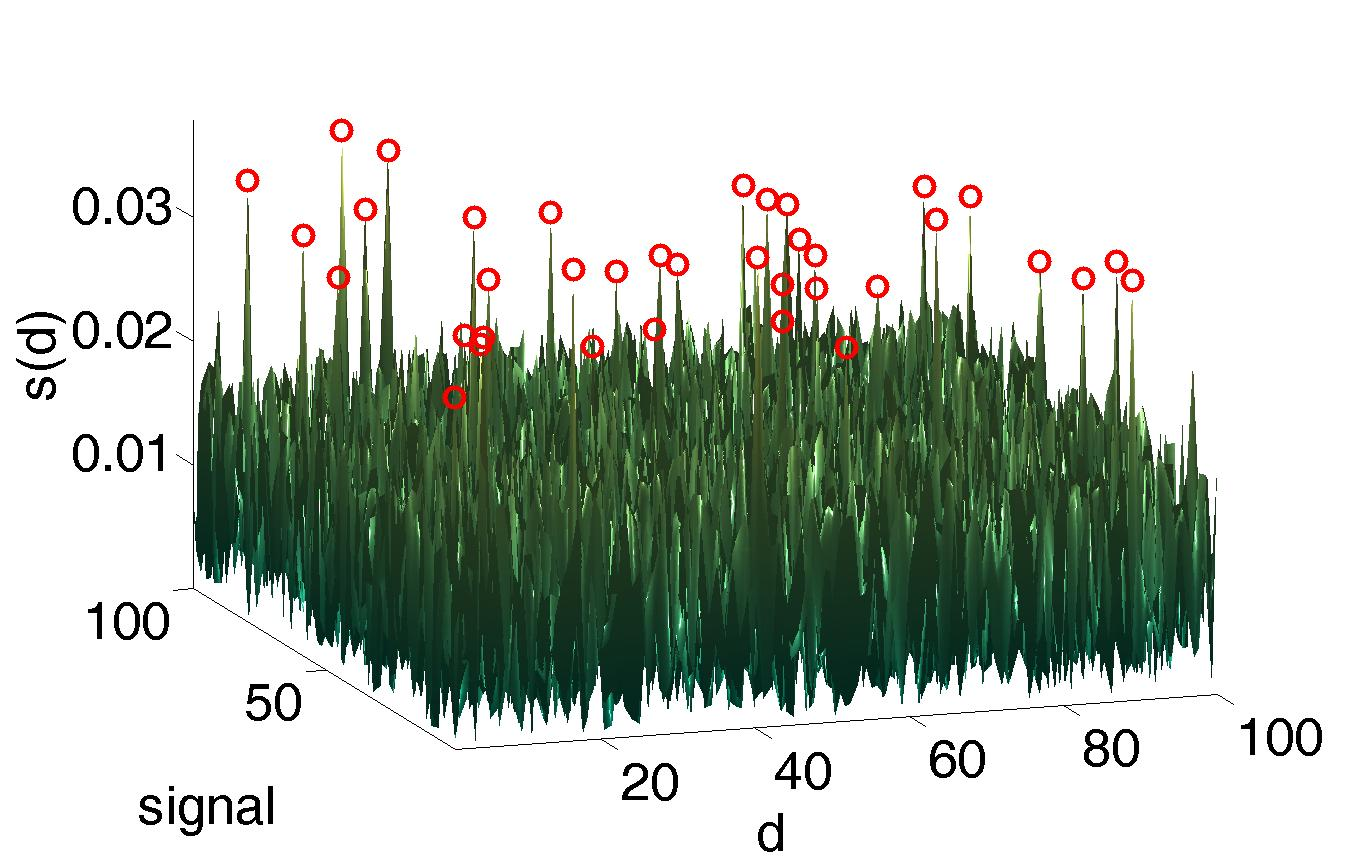
\includegraphics[scale=0.07]{randSignalSurfaceWithPeaks} % random signal
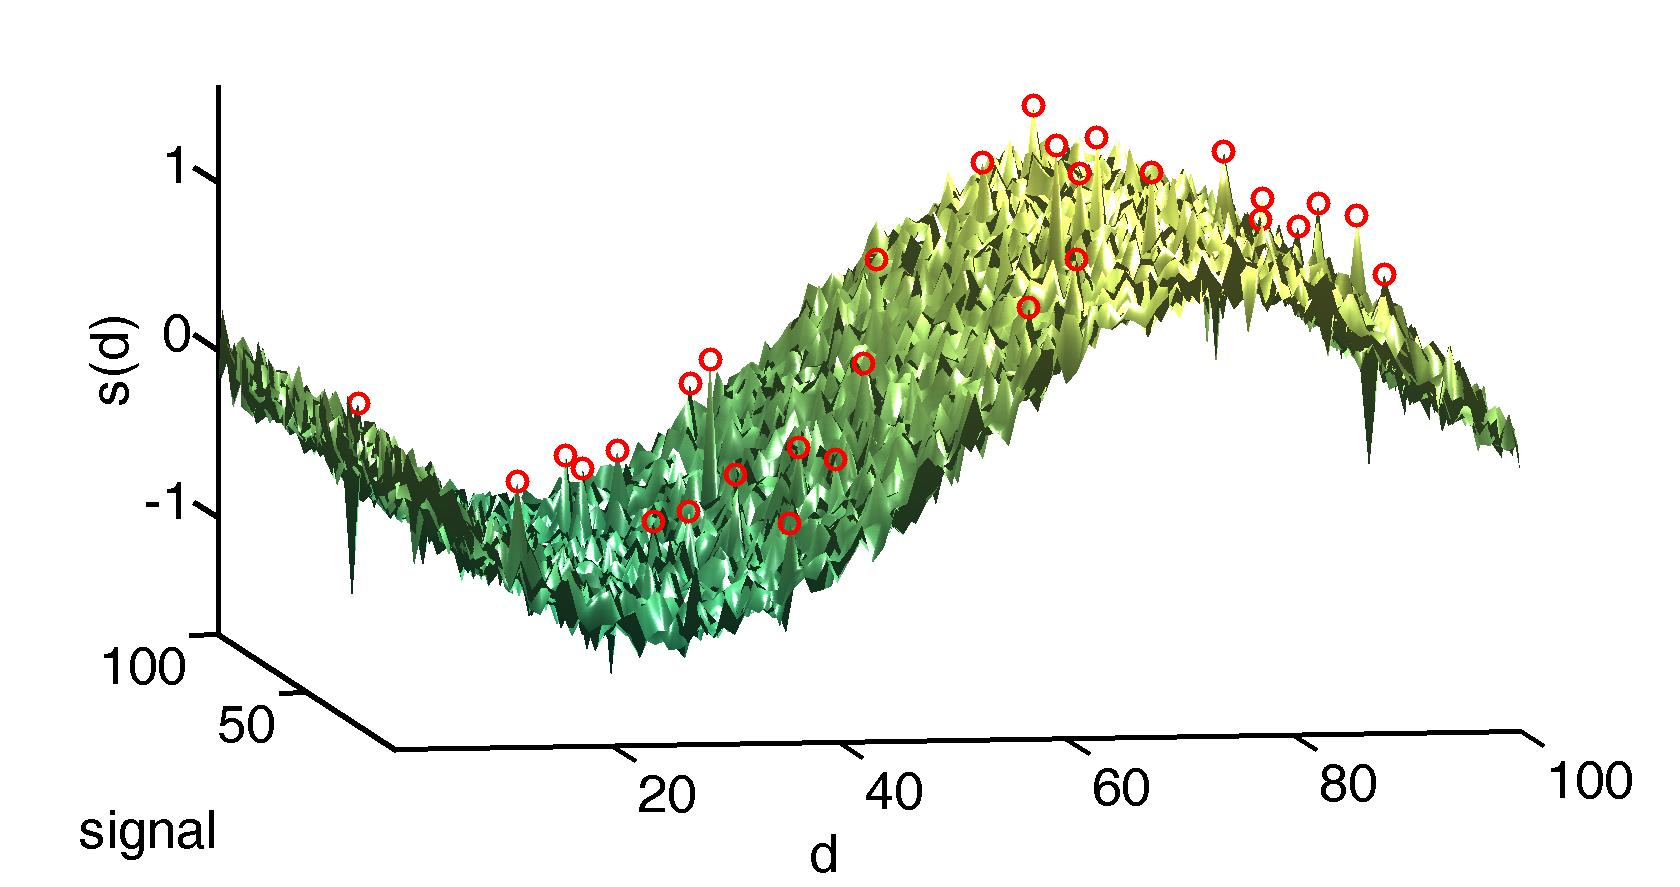
\includegraphics[scale=0.07]{sineSignalSurfaceWithPeaks} % sine signal
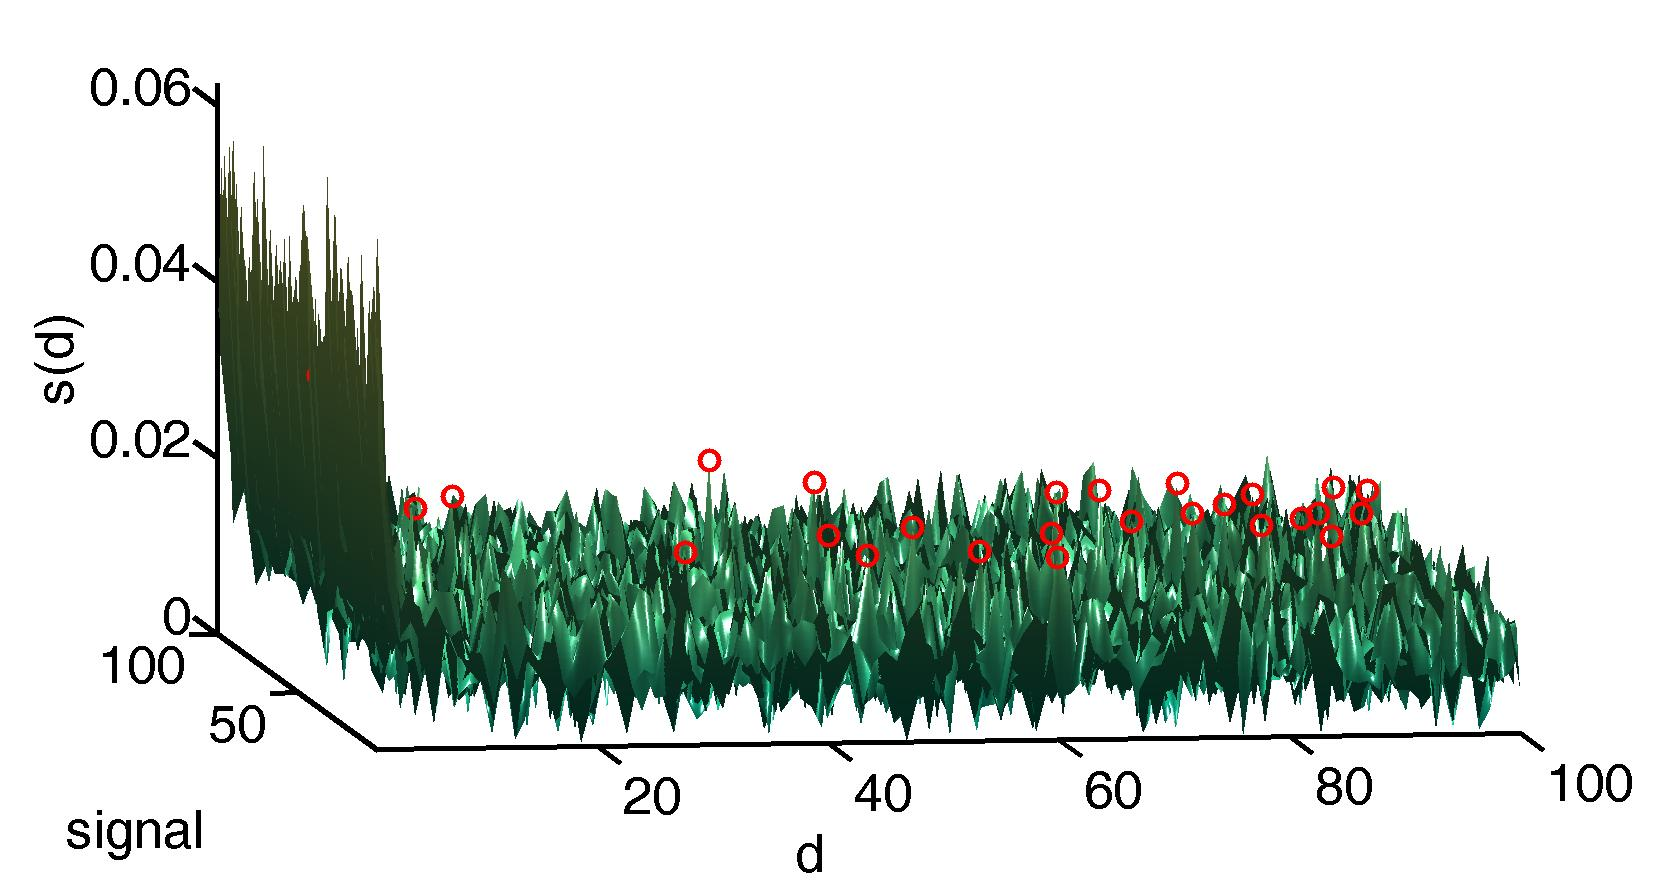
\includegraphics[scale=0.07]{gaussianChainSignalSurfaceWithPeaks} % gaussian chain 
\end{figure}
\begin{figure}[H]
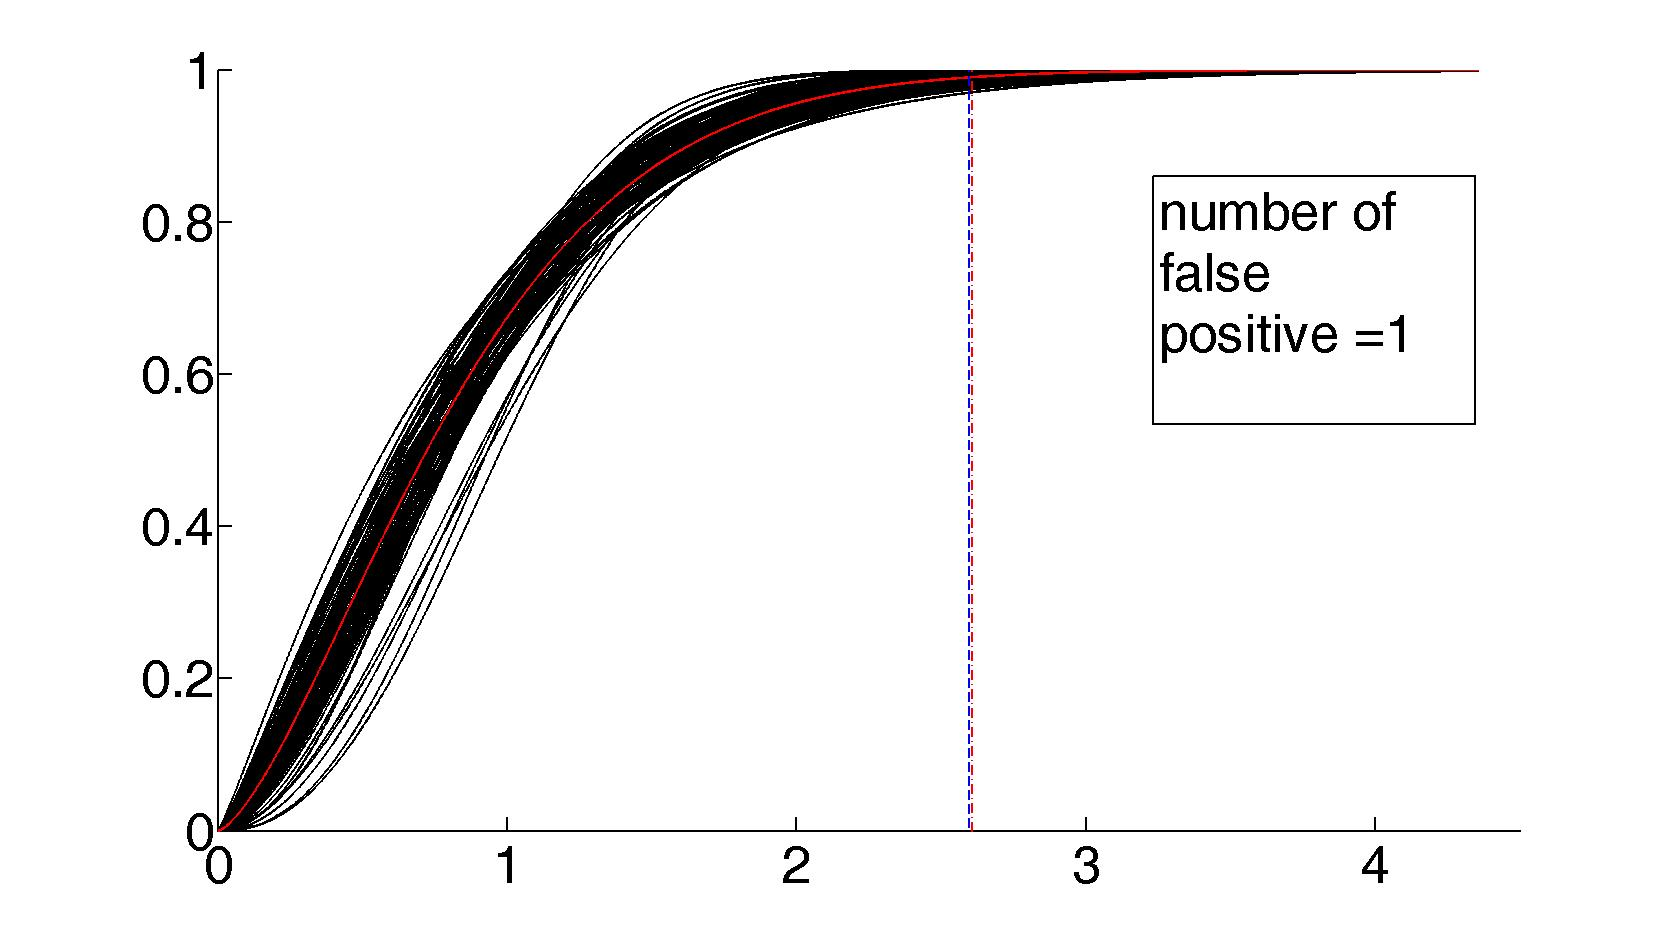
\includegraphics[scale=0.07]{randSignalZScoreDistributionWithThresh} % random signal
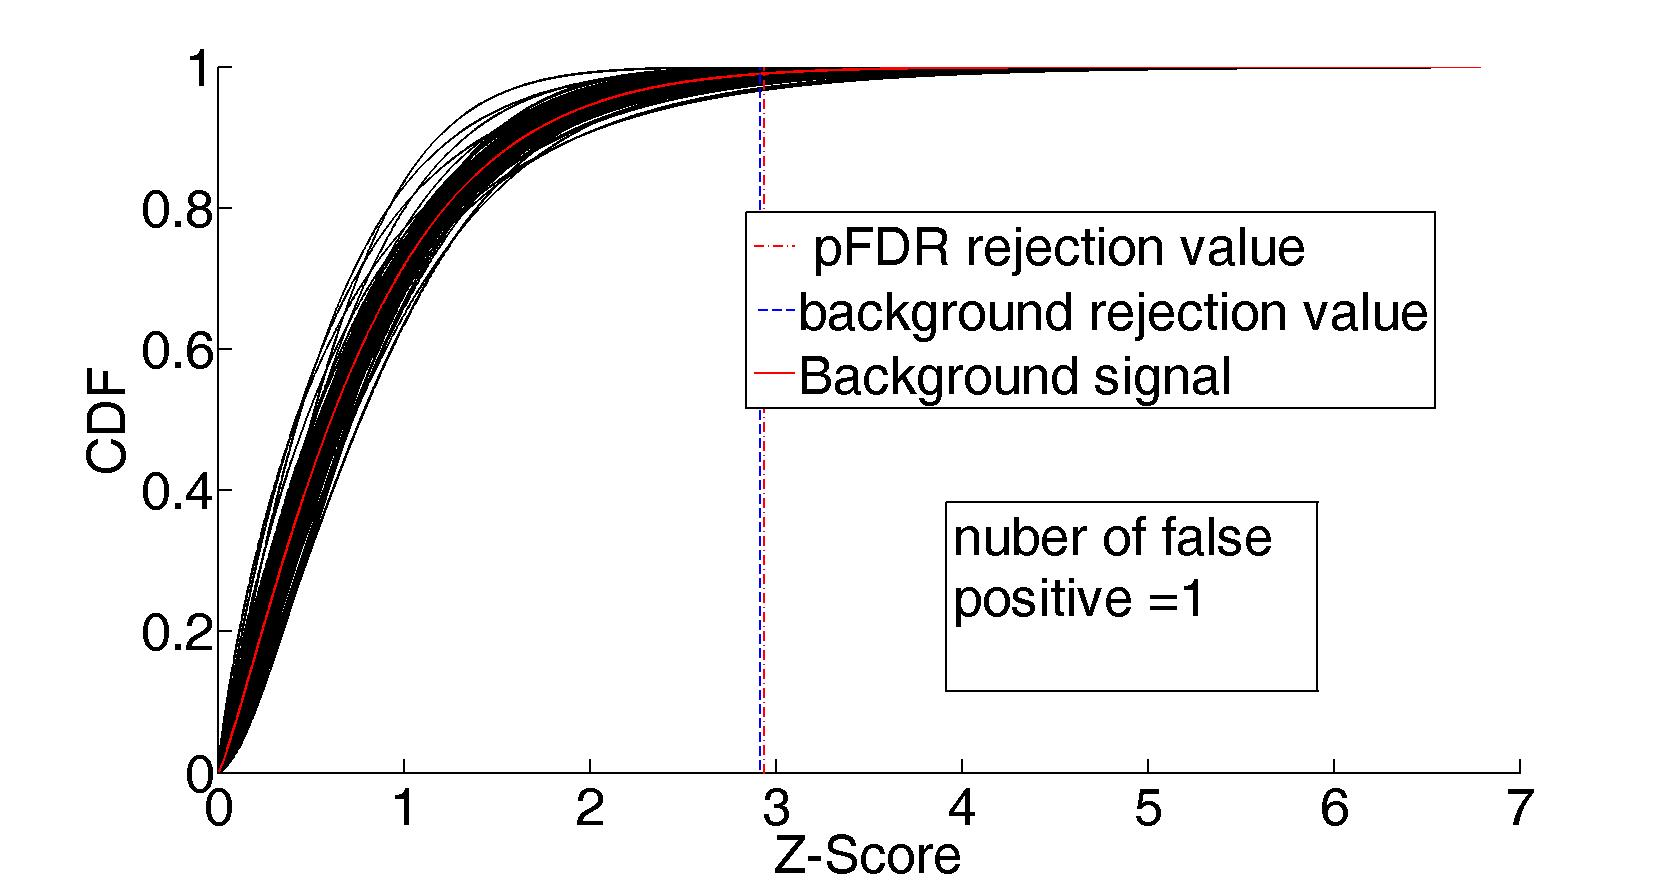
\includegraphics[scale=0.07]{sineSignalZScoreDistributionWithThresh} % sine signal
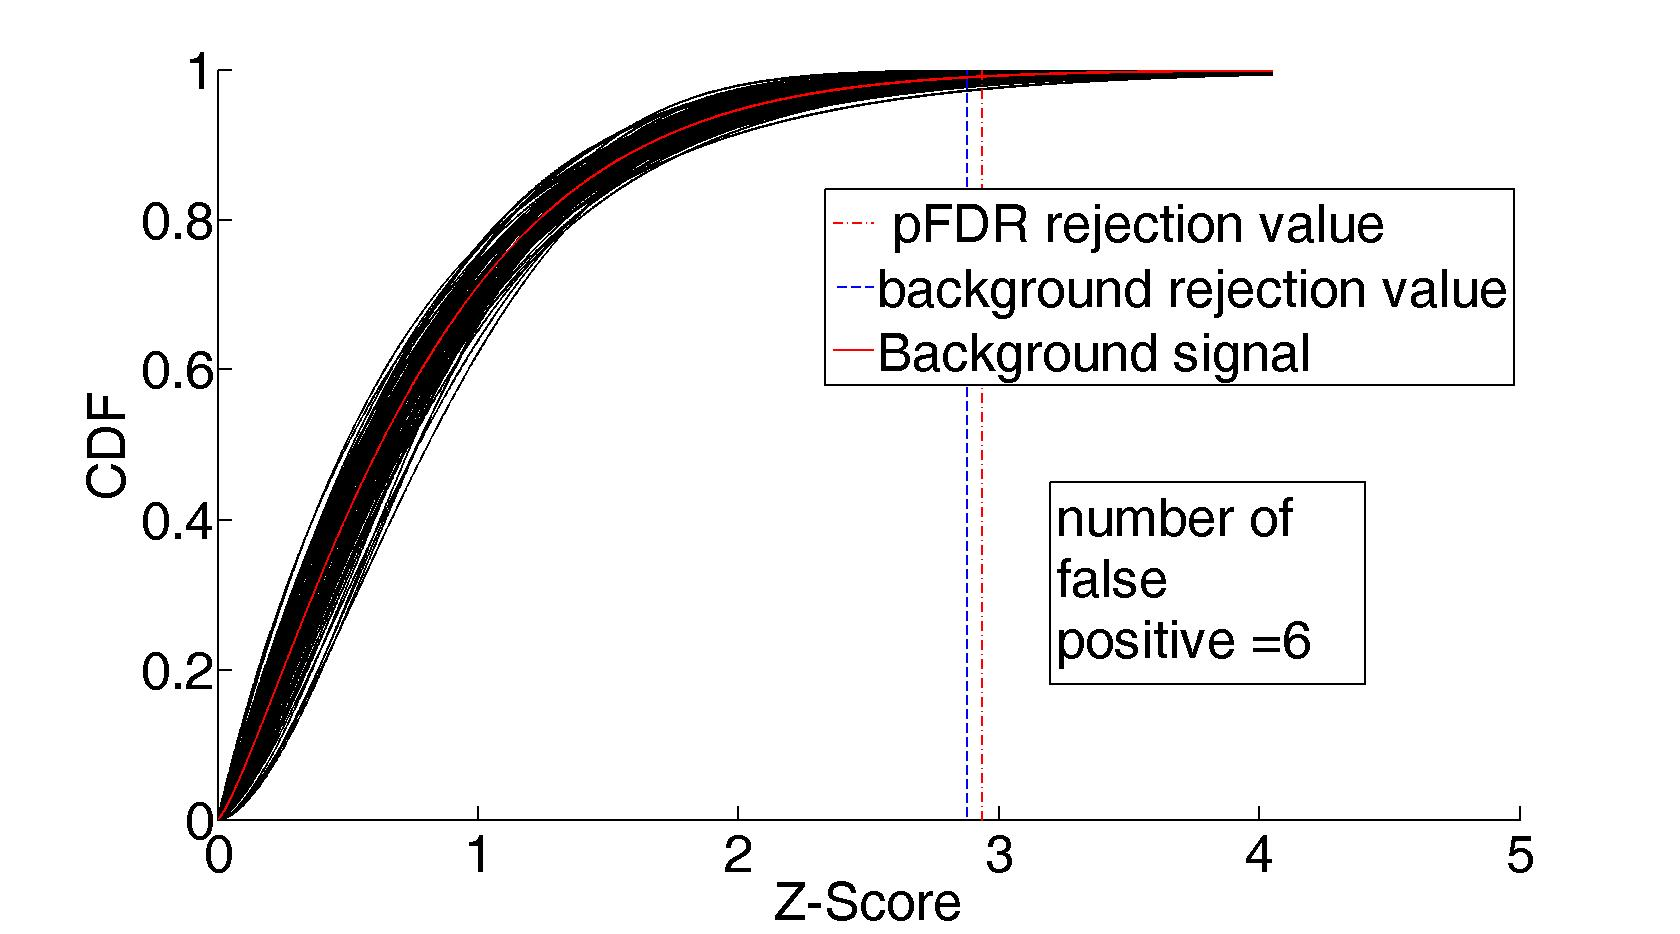
\includegraphics[scale=0.07]{gaussianChainZScoreDistributionWithThresh} % gaussian chain
\end{figure}
\begin{figure}[H]
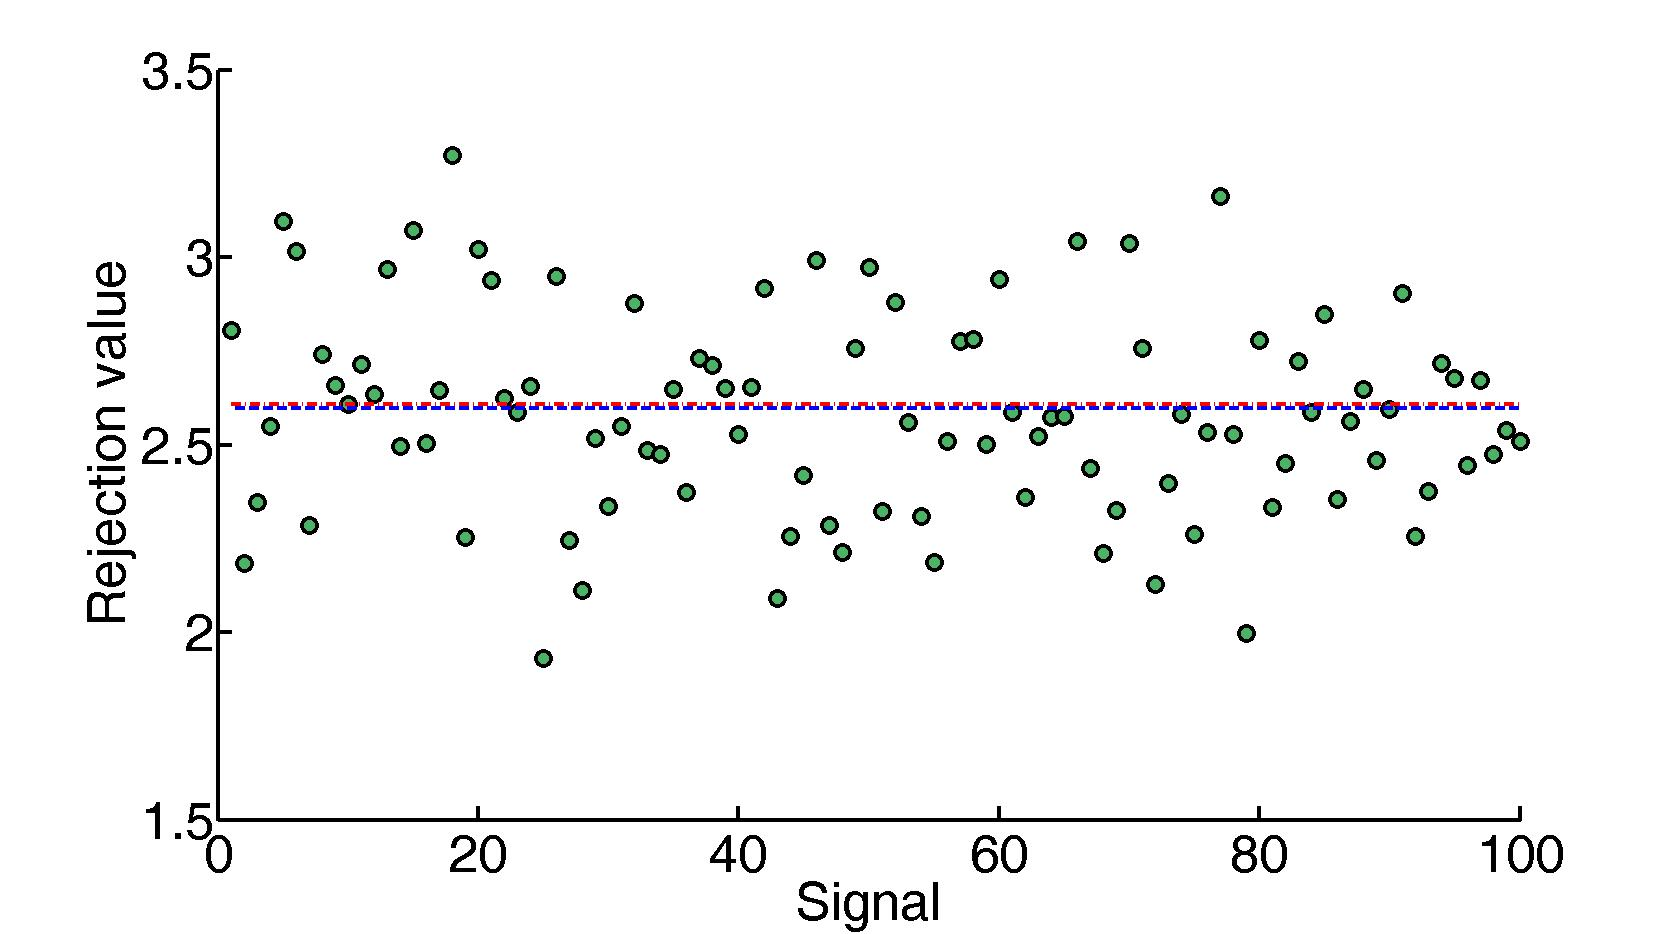
\includegraphics[scale=0.07]{randSignalRejectionDistribution} % random signal 
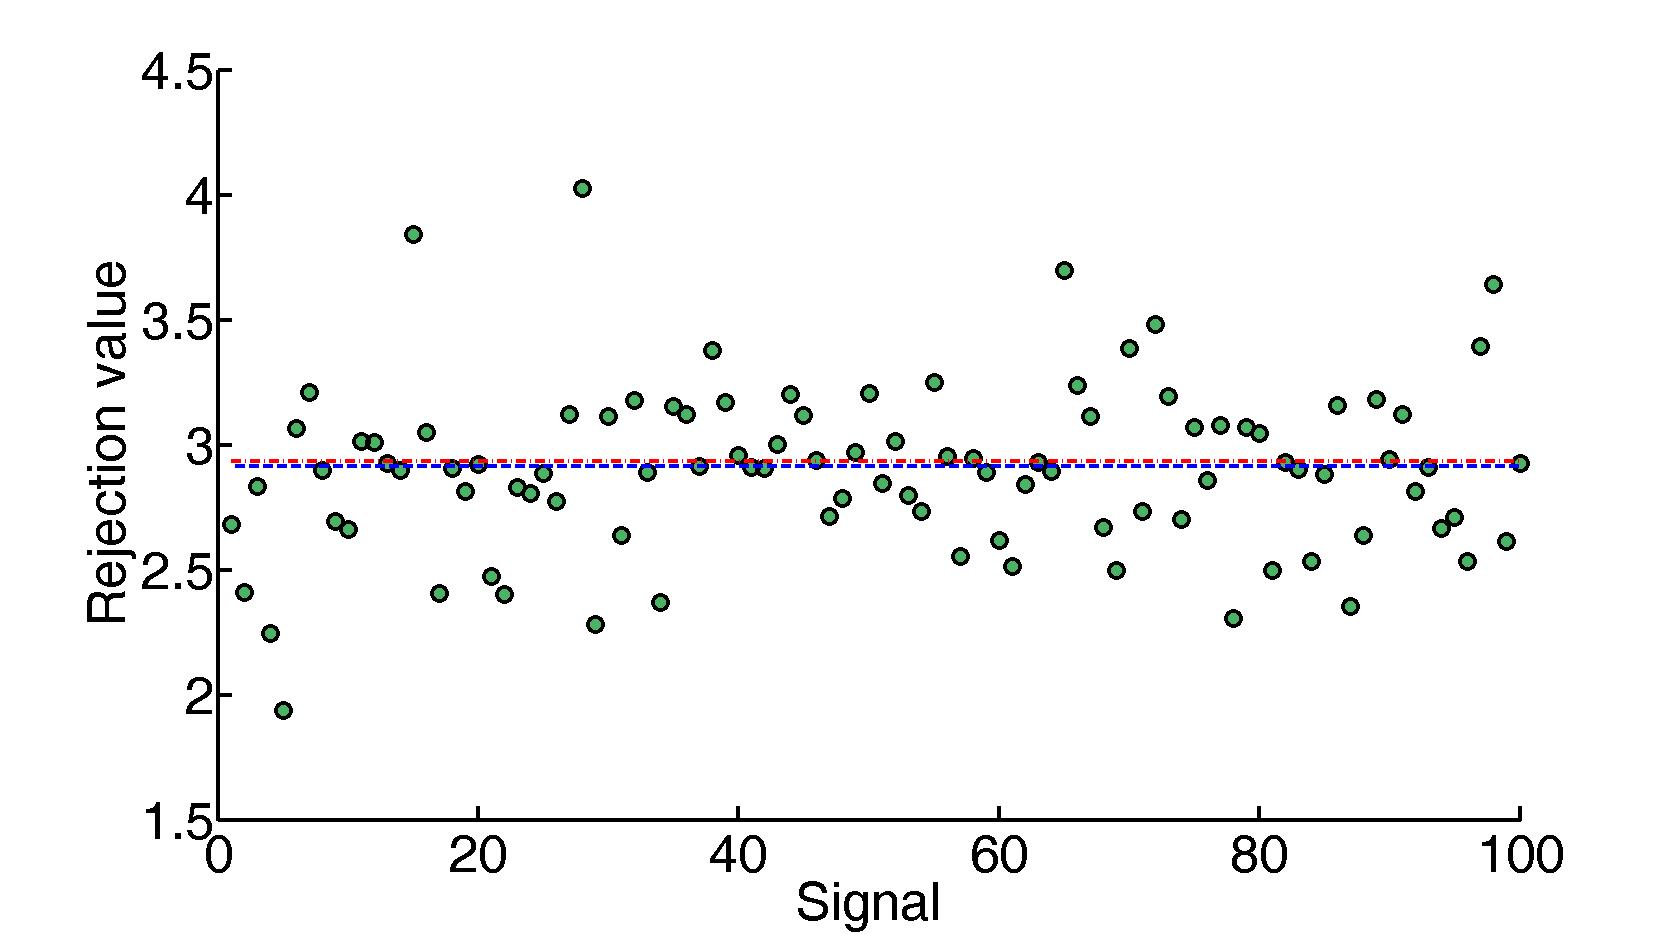
\includegraphics[scale=0.07]{sineSignalRejectionDistribution} % sine signal
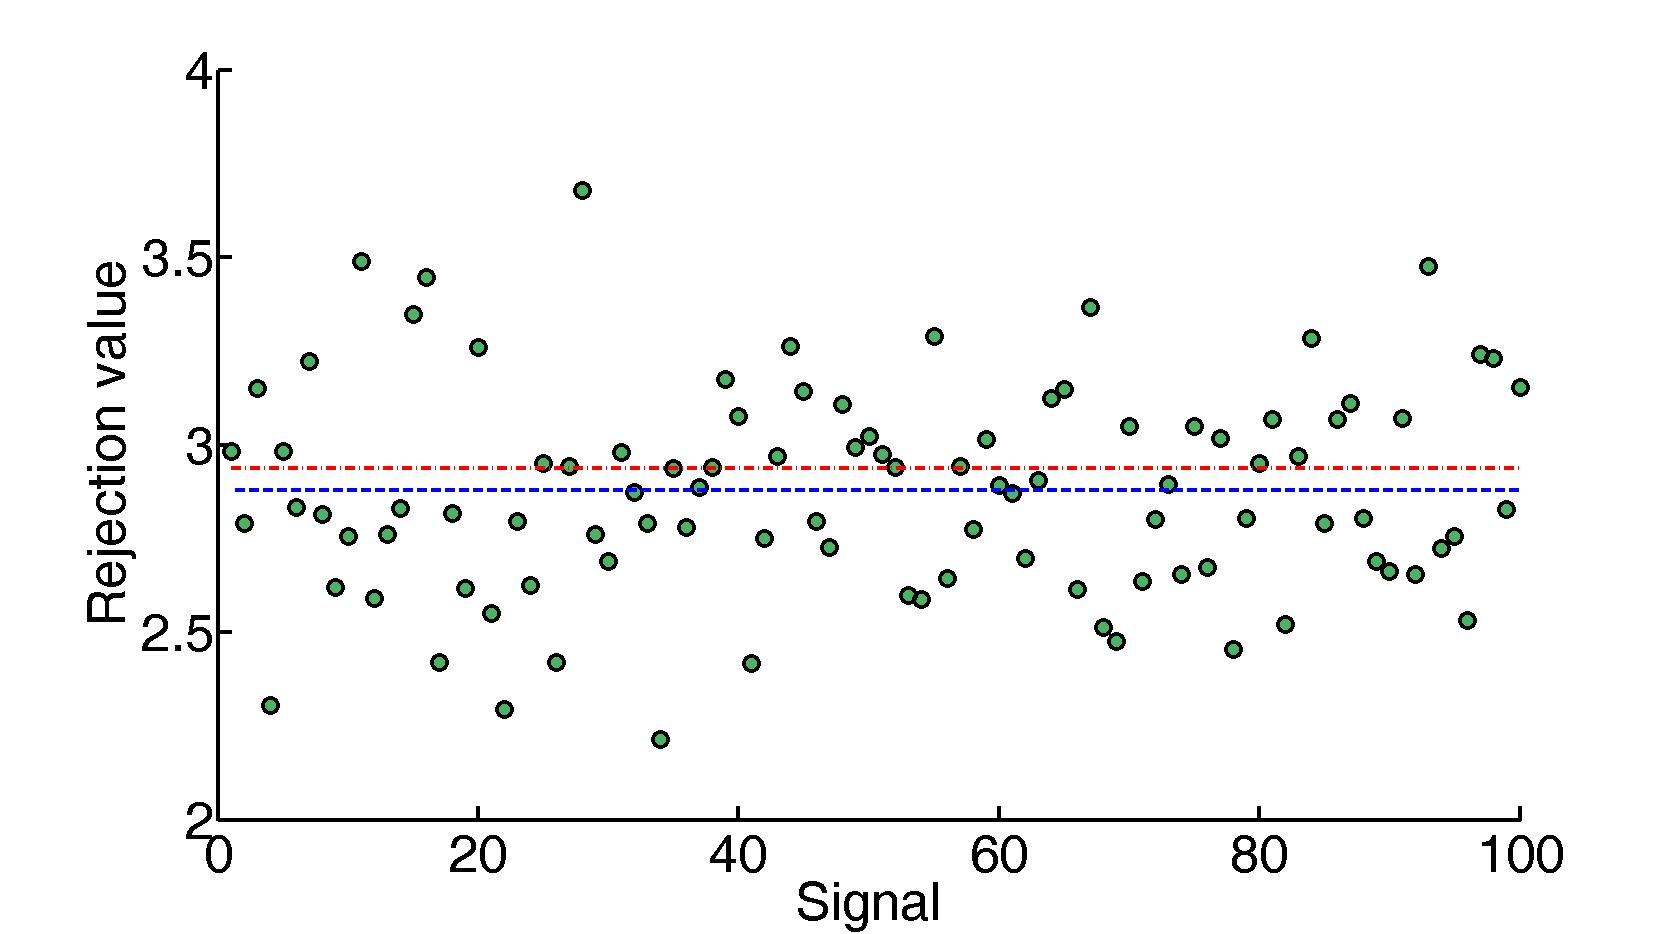
\includegraphics[scale=0.07]{gaussianChainSignalRejectionDistribution} % gaussian chain

\end{figure}

\end{frame}

\begin{frame}{Finding peaks of the 5C data}

\begin{figure}[H]
\includegraphics[scale=0.3]{tadDandENoraEtAl2012}
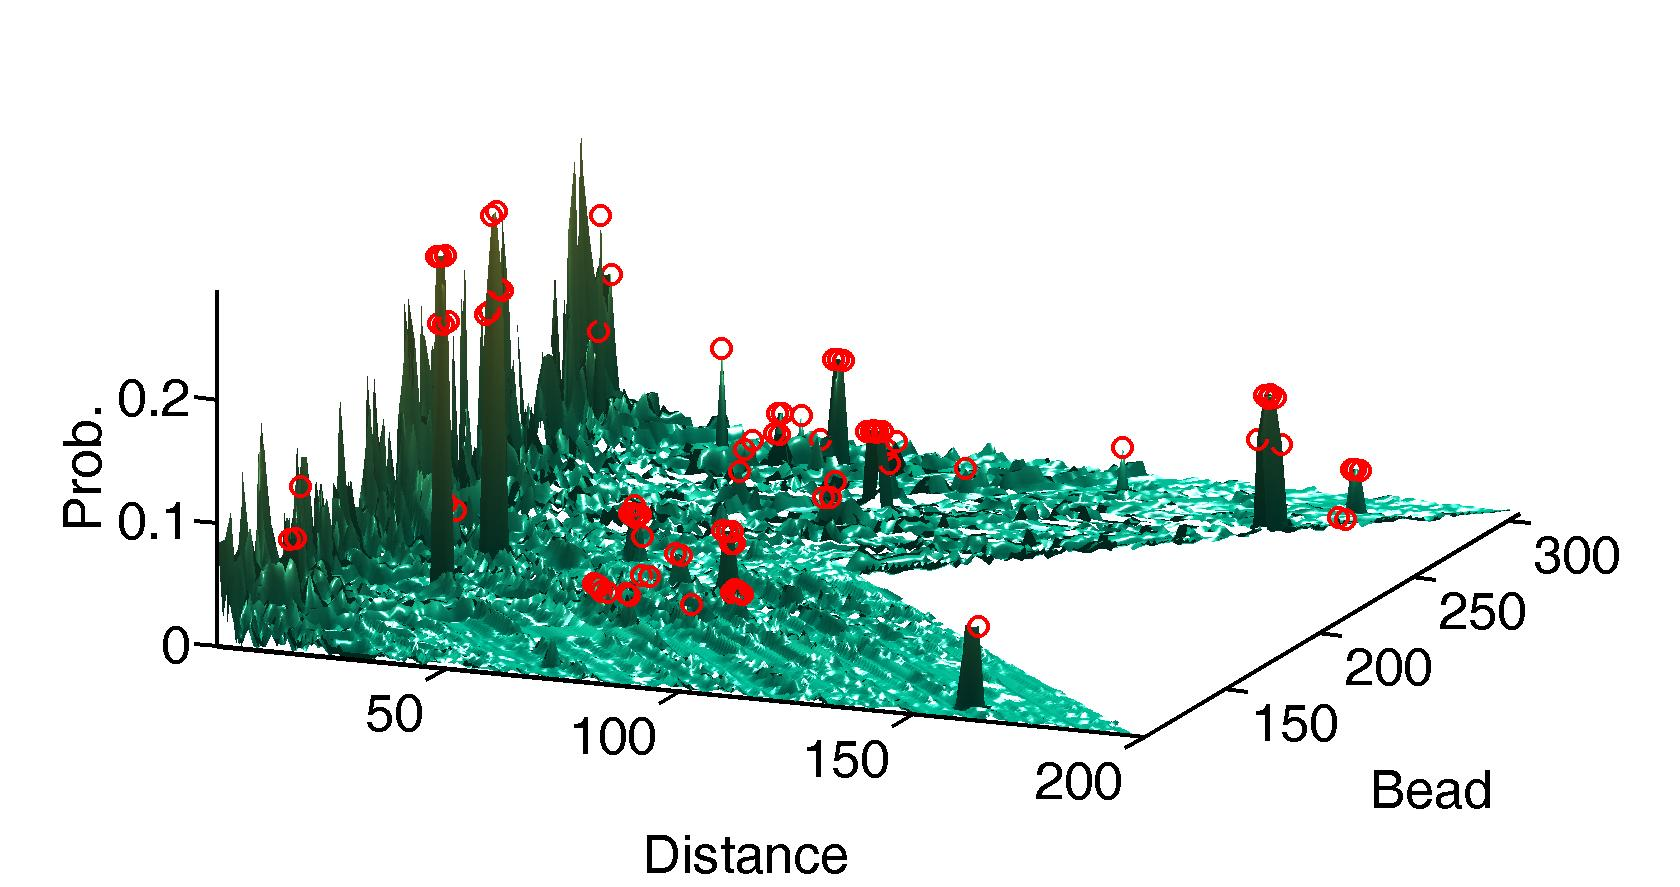
\includegraphics[scale=0.15]{tadESurfaceWithPeaks}
\end{figure}
\begin{figure}[H]
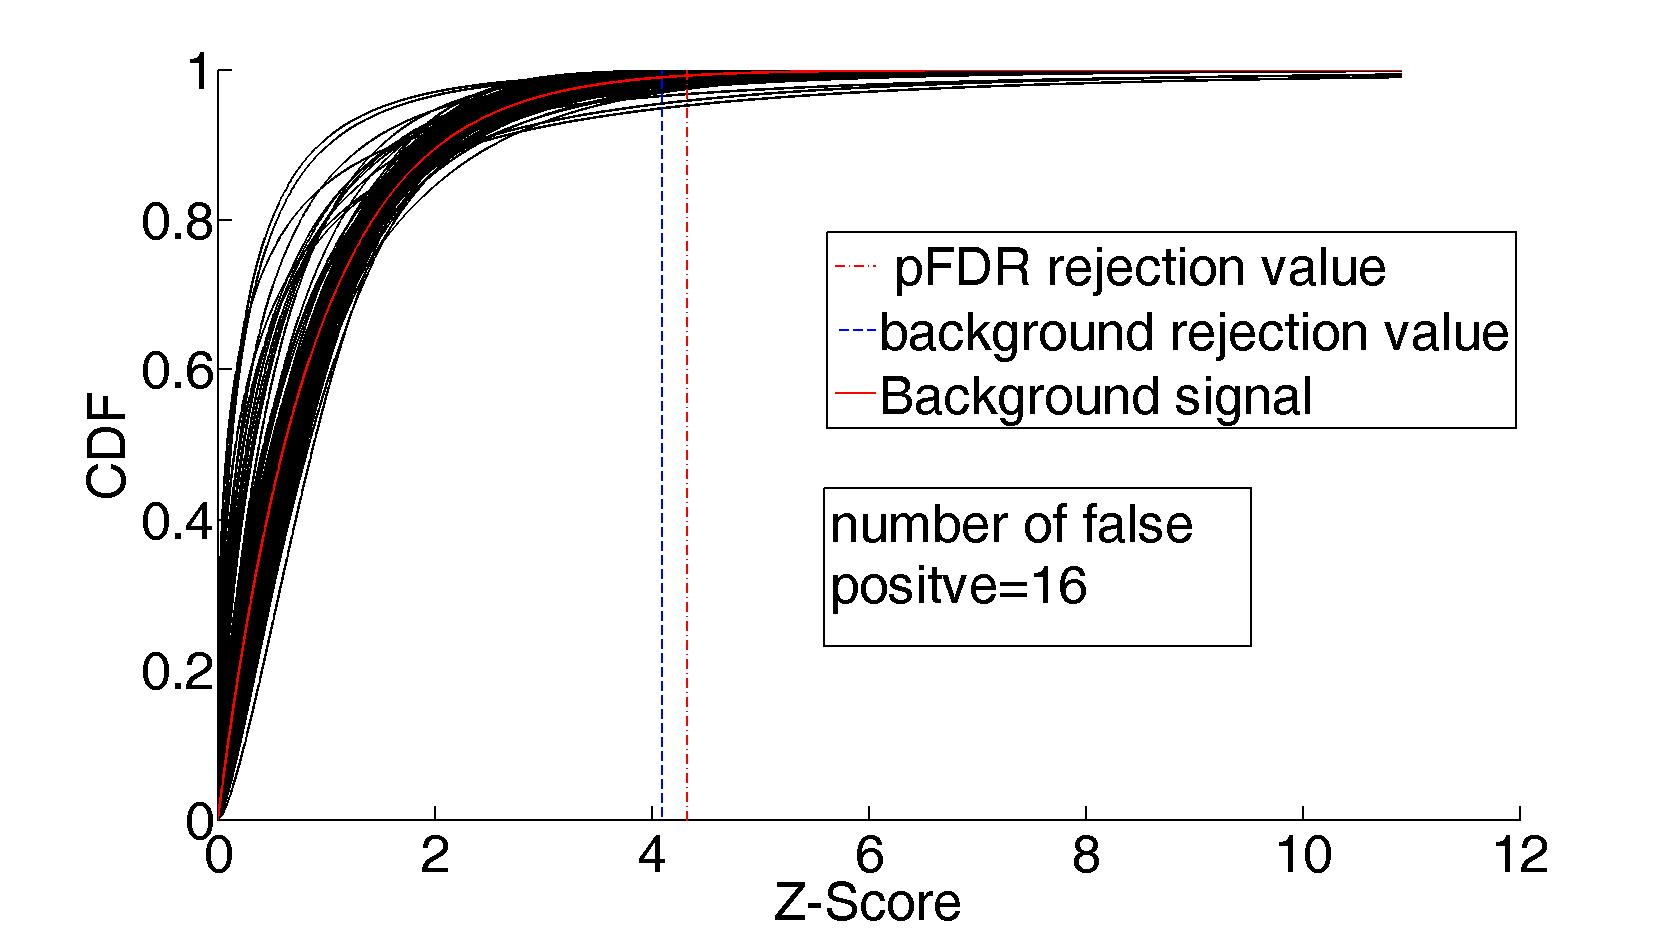
\includegraphics[scale=0.07]{tadEZScoreDistributionWithThresh}
\end{figure}
\end{frame}

\begin{frame}{From encounter probability to chromosome structure}
\begin{enumerate}
\item What do we do with the peaks after we've found them?
\item Assuming a Rouse model, one option is to connect with a spring any two beads corresponding to peaks.
\item If beads $i$ and $l$ correspond to a peak: 
\begin{figure}[H]
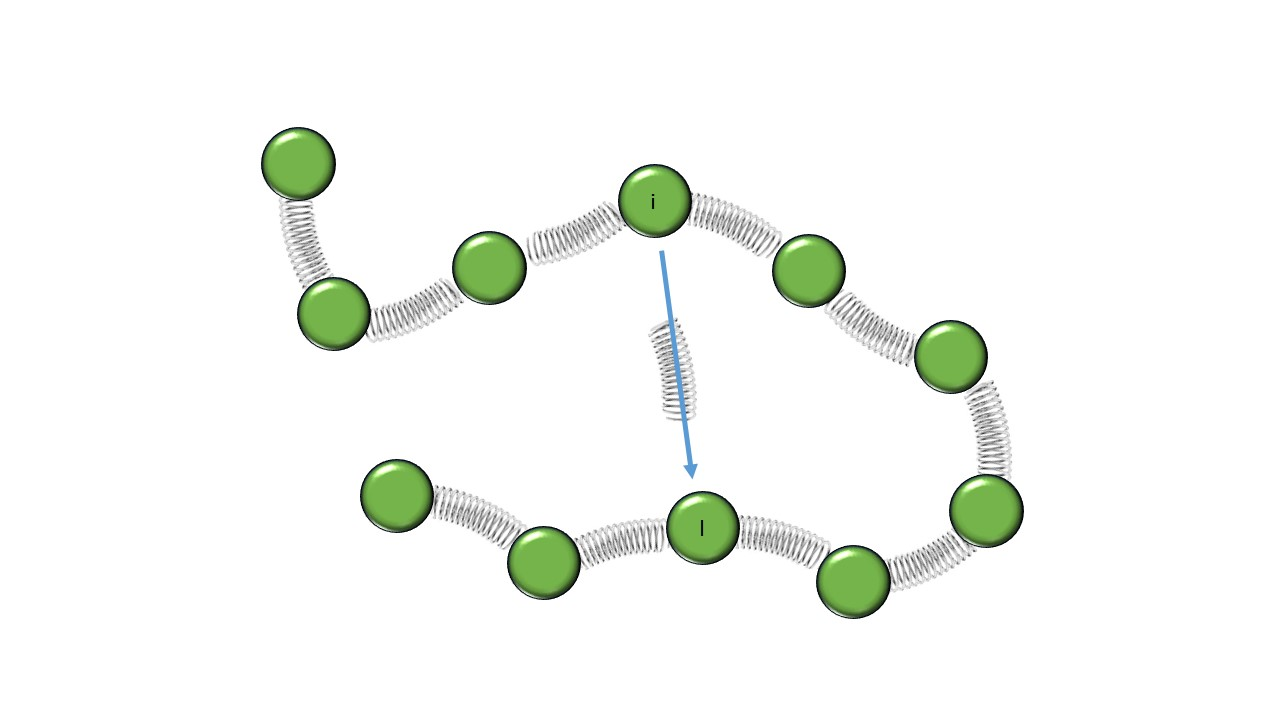
\includegraphics[scale=0.15]{connectBeadsCorrespondingToPeaks}
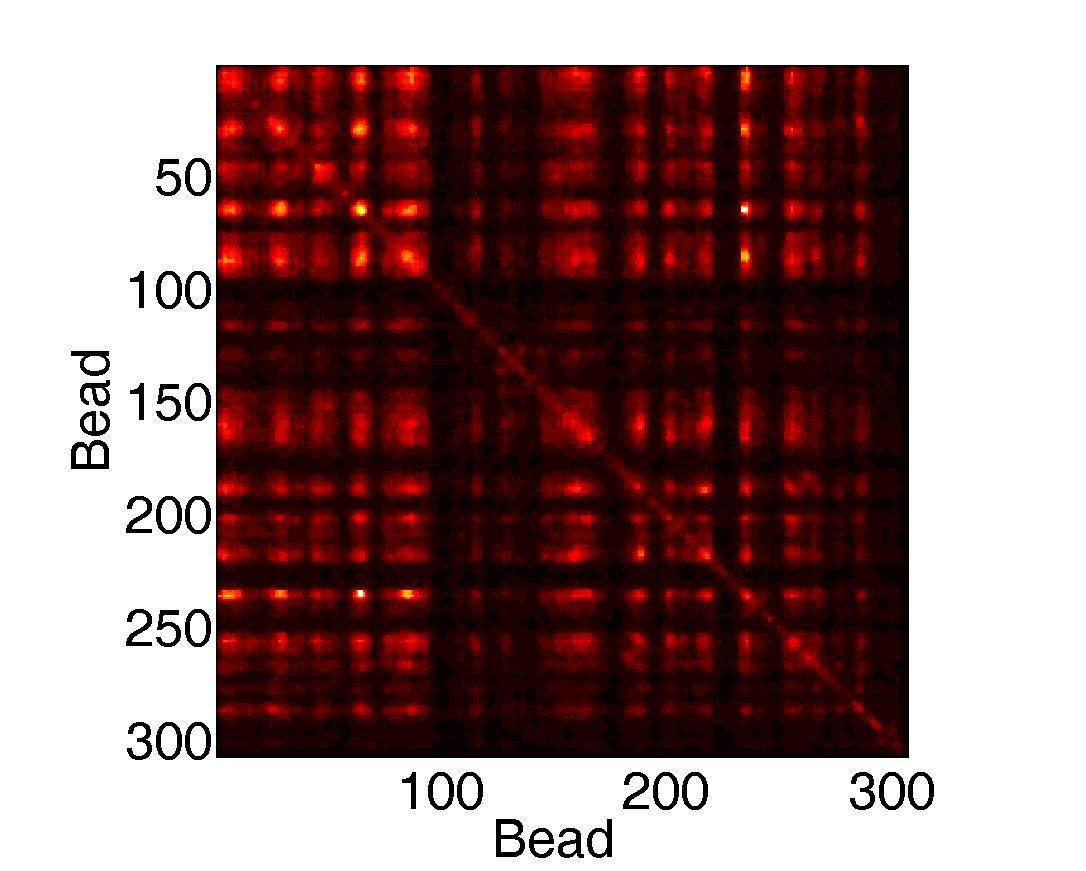
\includegraphics[scale=0.07]{EncounterHistogramLoopsCorrespondingToPeaksExperimentalData}
\end{figure}
\item The encounter histogram on the right does not look like the experimental data. 
\item The hight of the peak has to be taken into account. 
\end{enumerate}
\end{frame}

\begin{frame}{From encounter probability to chromosome structure}
\begin{enumerate}
\item Trivially, connecting beads, the distance along the chain shortens.
\begin{figure}[H]
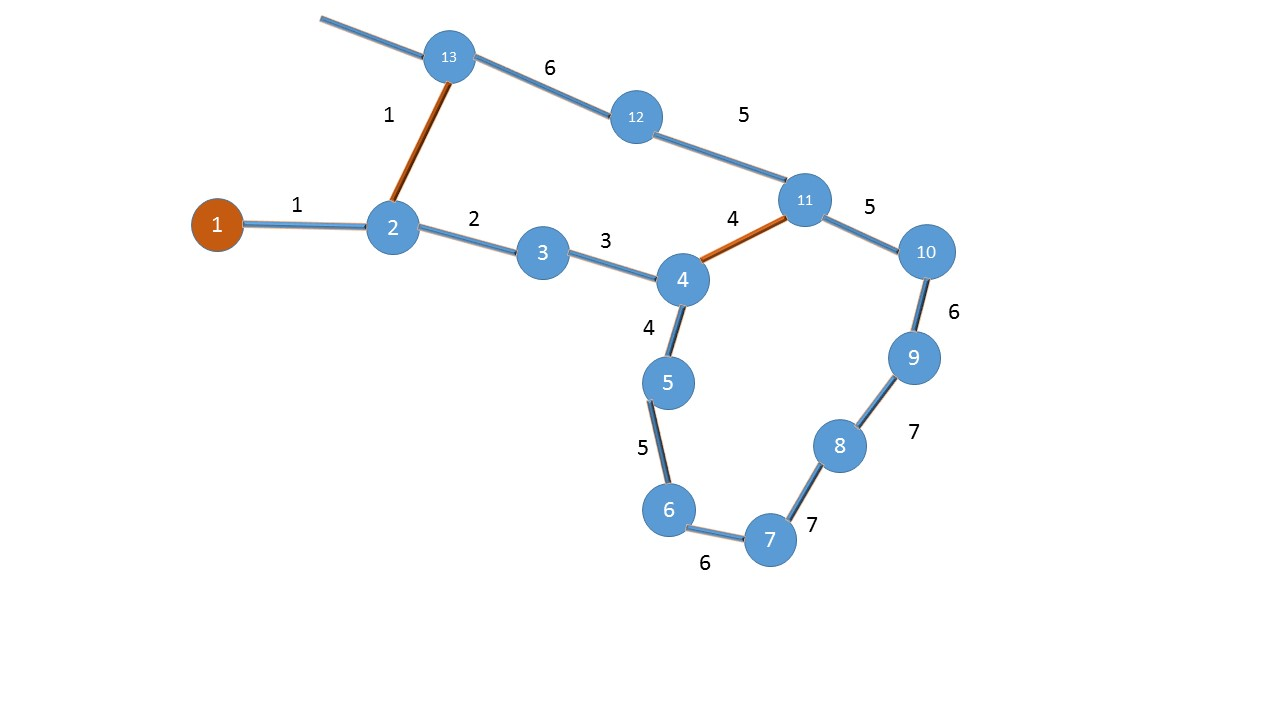
\includegraphics[scale=0.15]{connectedBeadsAndDistanceAlongTheChain}
\end{figure}
\item In the figure, distance along the chain from bead 1. Added connections marked in orange
\item The encounter probability should carry information about the distances between beads. 
\item Assuming a Rouse model, we know that $Pr(encounter(i,l))\sim dist(i,l)^{-1.5}$ in 3D. 
\end{enumerate}
\end{frame}

\begin{frame}{Projecting encounter Probabilities onto the encounter curve}
\begin{figure}[H]
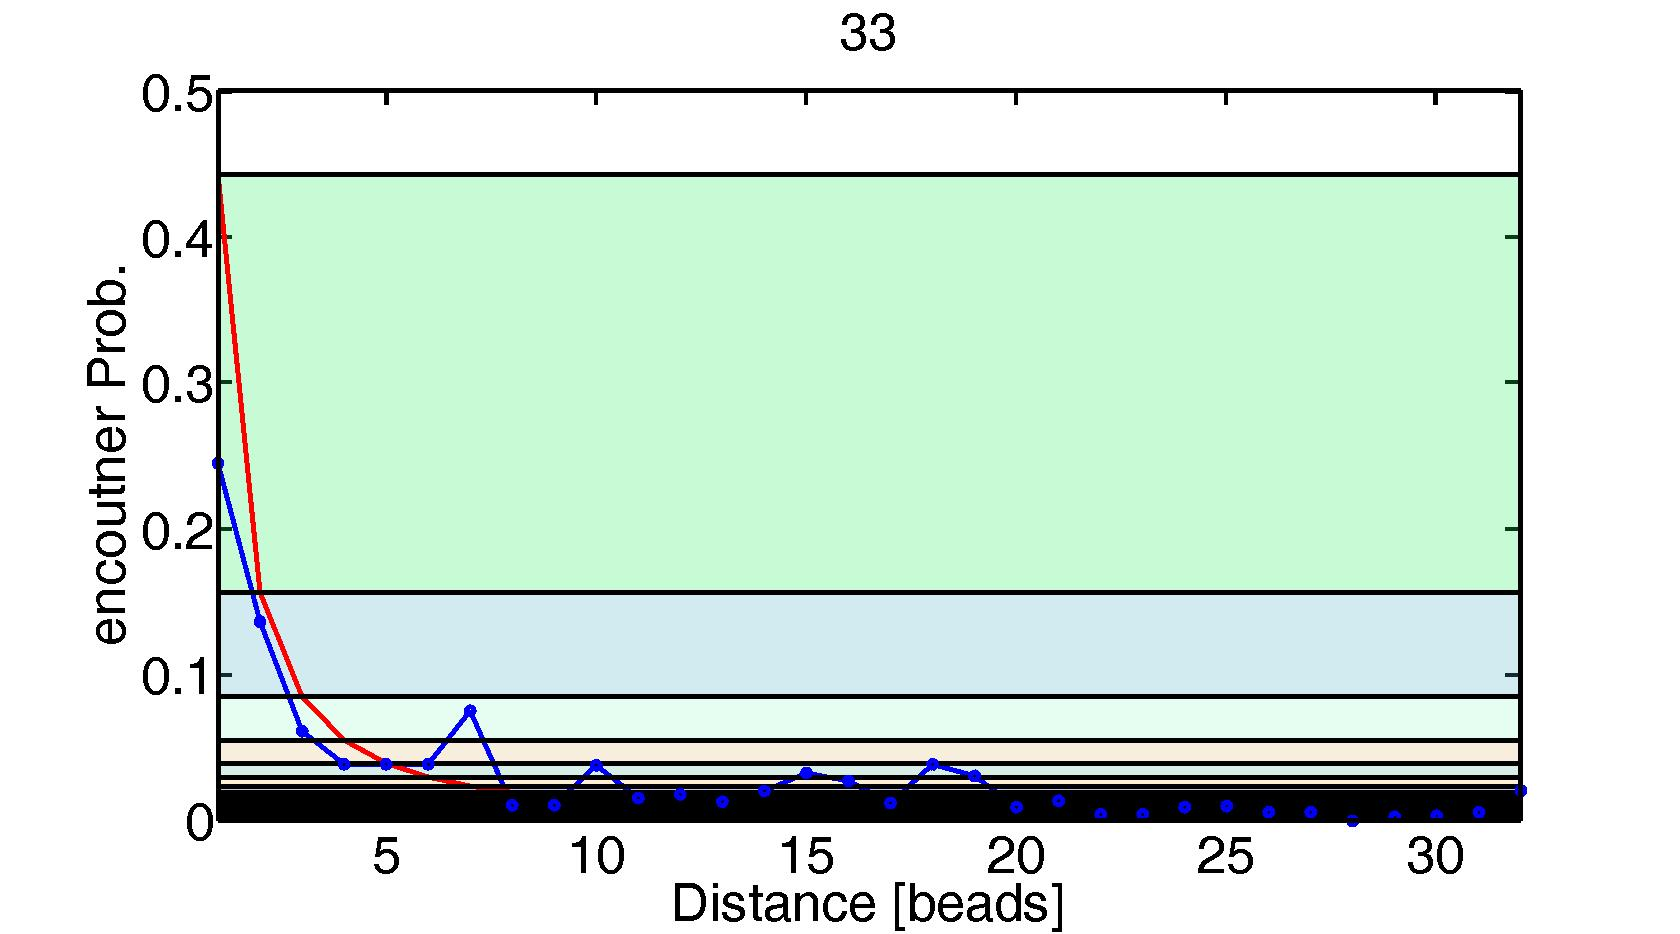
\includegraphics[scale=0.15]{encounterProbProjectedDist33}
\end{figure}
we see that the encounter probability at distance 7 for bead 33 corresponds to distance 3 under the assumption of the Rouse model.\\

We have enough data to discover the distances between beads under the assumption of a polymer model (data not shown)

\end{frame}


\begin{frame}{The spring constant corresponding to peaks}
What shall we do if the encounter probability is higher than the expected probability of the nearest neighbor?
\begin{enumerate}
\item For a Rouse chain the spring constant is $k=\frac{3k_BT}{b^2}$
\item We need to distinguish nearest neighbors encounter probability from encounter probability stemming from different spring constants.
\item The bead distance probability in 3D is $P(r)=\left(\frac{3}{2\pi b^2}\right)^{1.5}\exp\left(-\frac{3r^2}{2b^2} \right)$
\item setting $r=b$ for nearest neighbor, we get in steady state $P(b)=\left(\frac{3}{2\pi e b^2}\right)^{1.5}$.
\item estimating nearest neighbor probability, $\hat{P}(b)$ from the data \textit{without peaks}, and equating to $P(b)$, we get $ b^2 = \left(\frac{3}{2\pi e}\right)\hat{P}(b)^{1.5}$
\item Using the relation for the spring constant $k=\frac{k_BT}{b^2}$, we get $k=\frac{2\pi e k_BT}{3\hat{P}(b)^{1.5}}$
\item since $D=\frac{k_BT}{\xi}=\frac{k_BT}{6\pi\eta_s a}$, we get $k=\frac{4\pi eD \eta_s a}{\hat{P}(b)^{1.5}}$, if we have access to these parameters, otherwise
\item assuming we observe $P_{il}>\hat{P}(b)$ in the encounter probability signal, then the peak correspond to nearest neighbor and the estimation for $k$ is $ \frac{2k_BT\pi e}{3P_{il}}$
\end{enumerate}
\end{frame}

\begin{frame}{Summary}
\begin{enumerate}
\item I have presented the pFDR as means of controlling the error when searching for peaks in signals
\item The pFDR was applied on the CC data to eliminate false positive peaks. 
\item location of the peaks will be used when identifying parameters of the chain (spring constant)
\item future work will include incorporation of different spring constant and simulations with heterogeneous polymer.  
\end{enumerate}
\end{frame}
\end{document}